%In this report we apply regression and classification to the "Letter Image Recognition" dataset
\chapter*{Regression}
\setcounter{chapter}{1}
\section*{1.1 Problem}
\setcounter{section}{1}
Let D denote our data set that contains N observations:
\begin{center}
$D = \{( \textbf{x}_i ,y_i ) | i = 1, 2, \dots, N\}$
\end{center}
Each $\textbf{x}_i $ corresponds to the set of attributes of the $i$-th observation and $y_i$, corresponds to the target variable. \\

Regression is the task of learning a target function $f$ that maps each attribute set $\textbf{x}$ into a continuous-valued output $y$. In particular, according to our dataset, the continuous-valued output corresponds to the letter index. 
Thus, the goal for our  regression problem, is to find a target function, which describe the letter index, that can fit the input data with minimum error. The error function for a regression task will be expressed in terms of squared error.\\

The idea is to set an index for each letter (for example $A=2, B=1 ... , Z = 25$) and then apply linear regression. 
If we apply linear regression for the whole data set (consider all the letters, equal to 26 classes) that will never work, linear regression is simply not sufficiently flexible,for instance, to understand that the differences in pixel intensities in $a, b, c$ should result in $y = 1, 2, 3$. Suppose $x_a$ corresponds to the input of a and $x_c$ the input of c. Then suppose you have trained the weights $w$ such that:
\begin{enumerate}
\item []$1 = x_a * w$
\item []$3 = x_c * w$
\item []it now follows that $2 = \frac{(x_a + x_a)}{2}* w$\\
\end{enumerate}

That said, we are going to solve two different linear regression problem:
\begin{enumerate}
\item Considering a subset of our data corresponding to two letters. Then we have a proper two-class problem
\item Applying 1 out of $K$ coding where $K=26$. We consider the one-against-rest scheme, where multiple classes are handled by decomposing the problem into $K$ binary problems, where $K$ is the number of classes. We train $K$ classifiers, each fitted to classify one class against the rest of the classes lumped together.
\end {enumerate}

\section*{TWO-CLASS LINEAR REGRESSION}

\section*{1.2 Forward selection}
\setcounter{section}{2}
We apply linear regression with forward selection considering a subset of data of two classes, where class 0 corresponds to the letter $A$ while class 1 corresponds to the letter $C$.Since our output are purely binary ($y \in {0,1}$), we use logit function which maps the output in the regression analysis to the range (0,1). To measure how well we can predict the the two letters, we will use the squared error between the true and the estimated error. In our estimation we  use two level of cross-validation. On the outer level, we use 5-fold cross-validation  to estimate the performance of our model computing the squared error averaged over 5 test sets. On the inner level, we use 10-fold cross-validation to perform sequential feature selection. Figure 1.1 shows that the most commonly selected features for letter recognition are width, x-bar, x2bar, y2bar, xy2br, xegvy, yegvx.


\begin{figure}[htbp]
\center
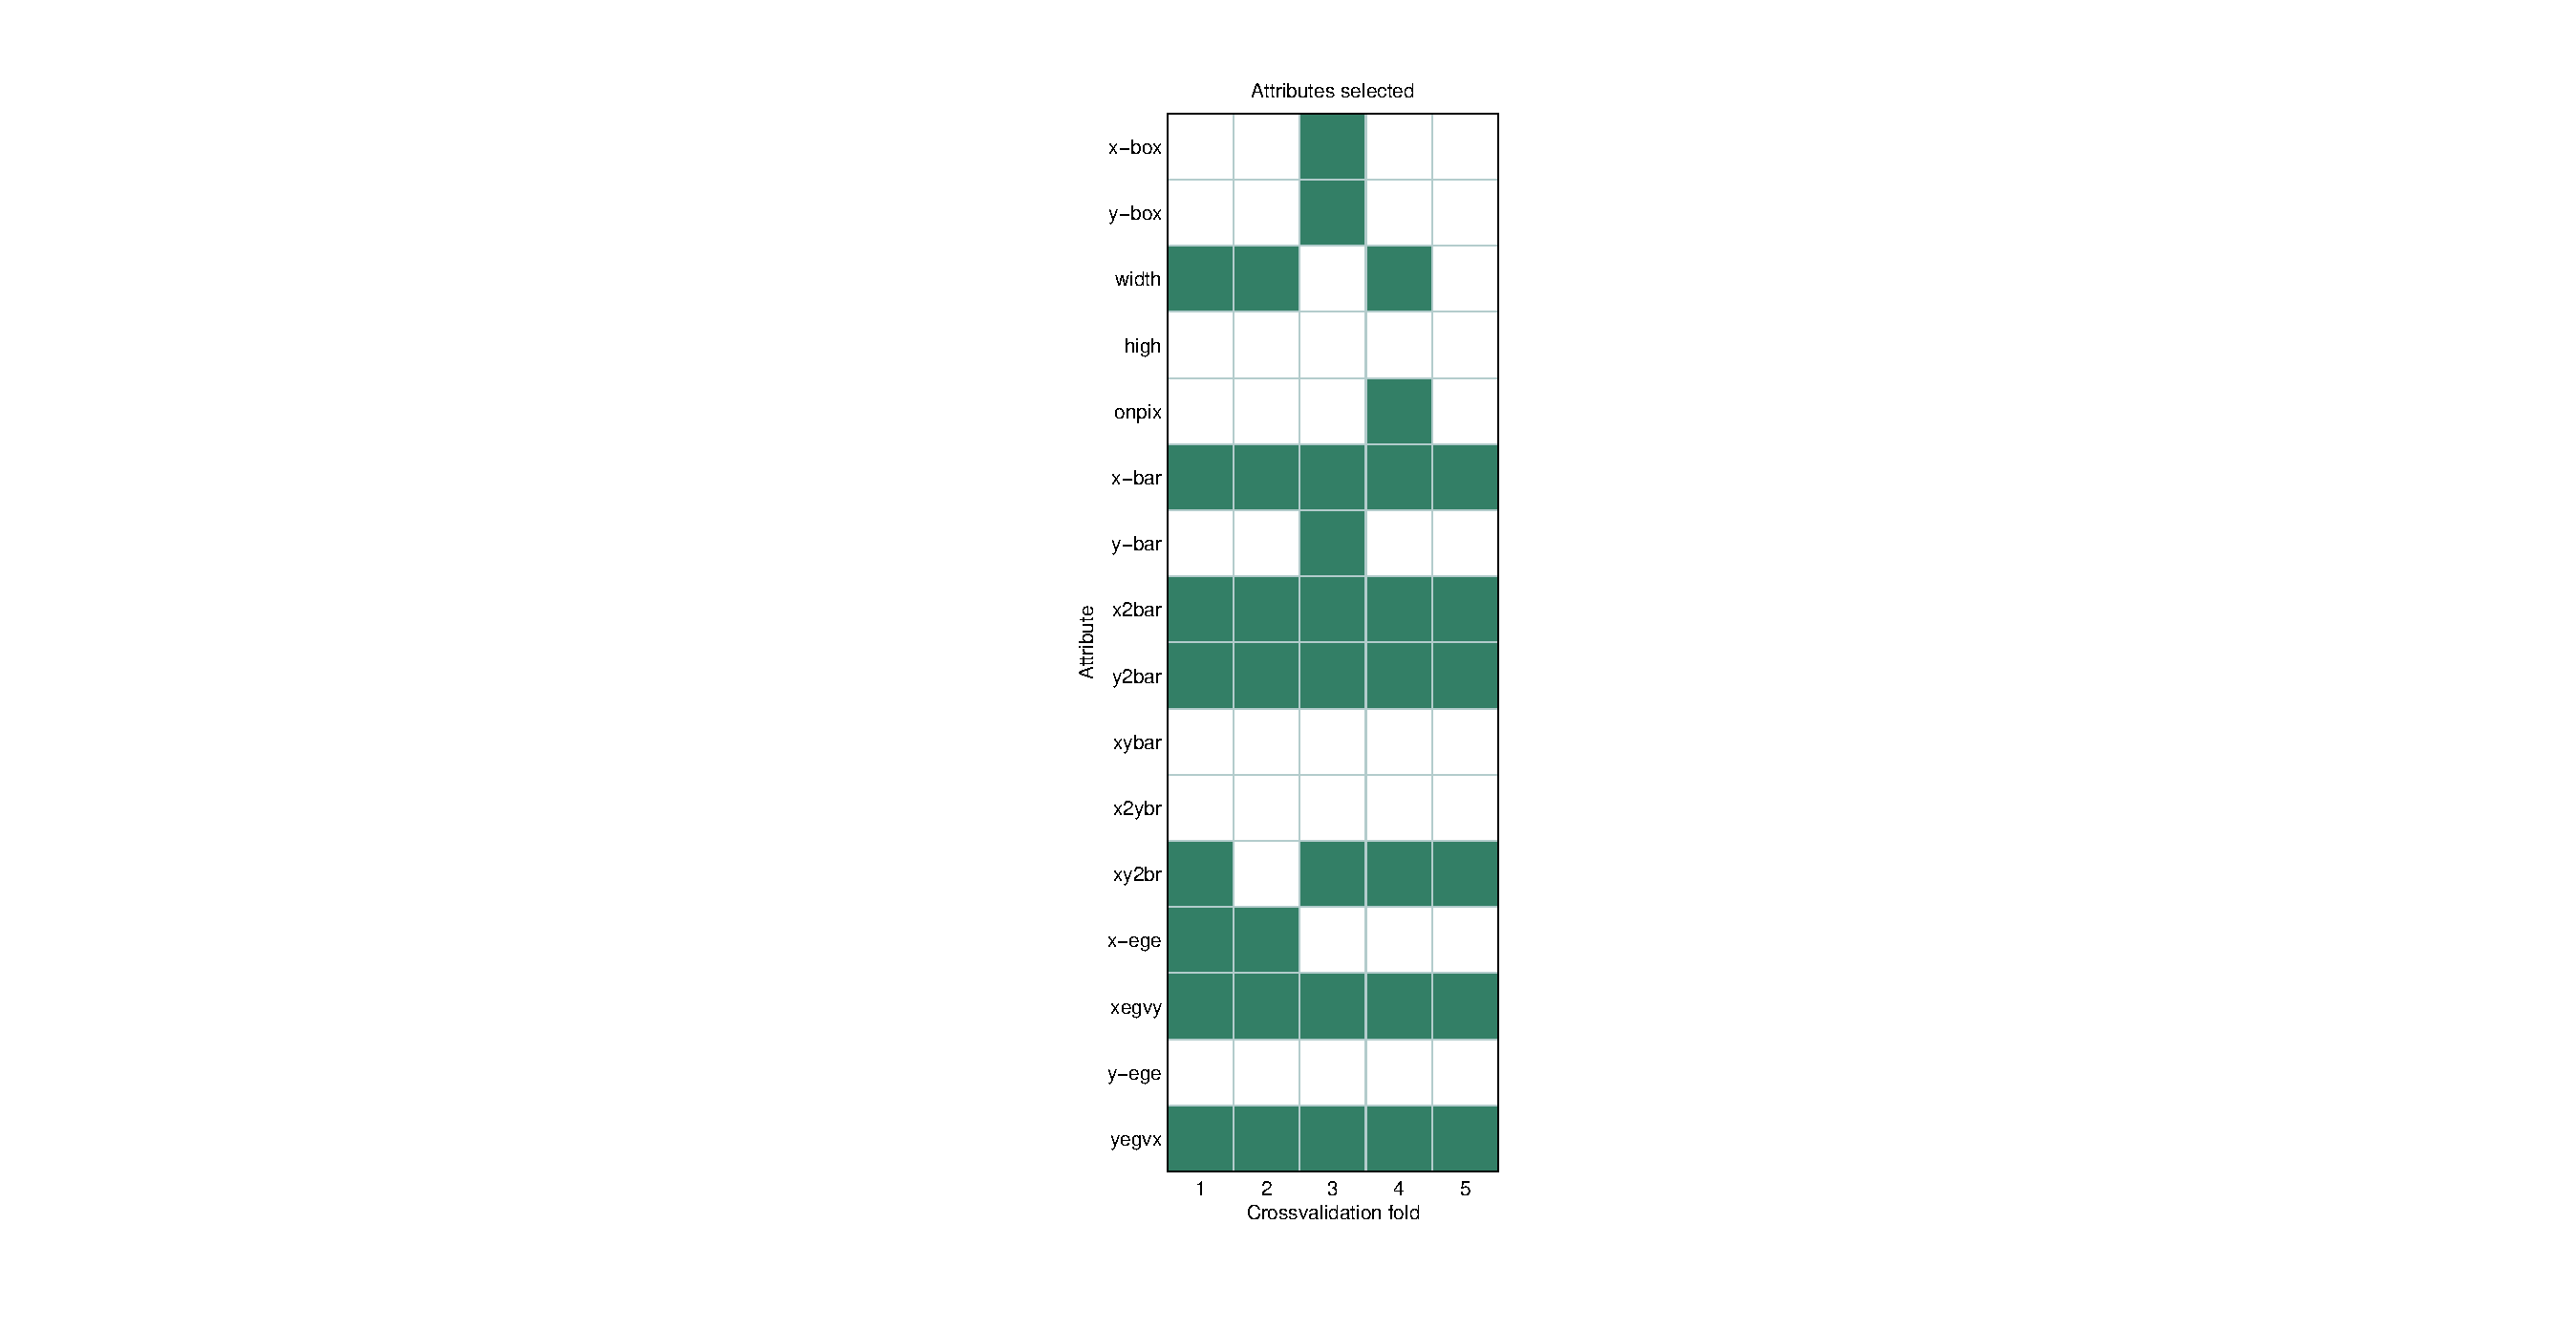
\includegraphics[width = 0.9\textwidth]{figure_p2/r1.eps}
\caption{Linear regression with forward selection, attributes selected for all folds}
\end{figure}

The fold which requires the less number of feature for the linear regression is fold number 5. Figure 1.2 shows feature selection and crossvalidation error for the fold 5. We can see that the minimum squared error is reached with only six attributes.

\begin{figure}[htbp]
\center
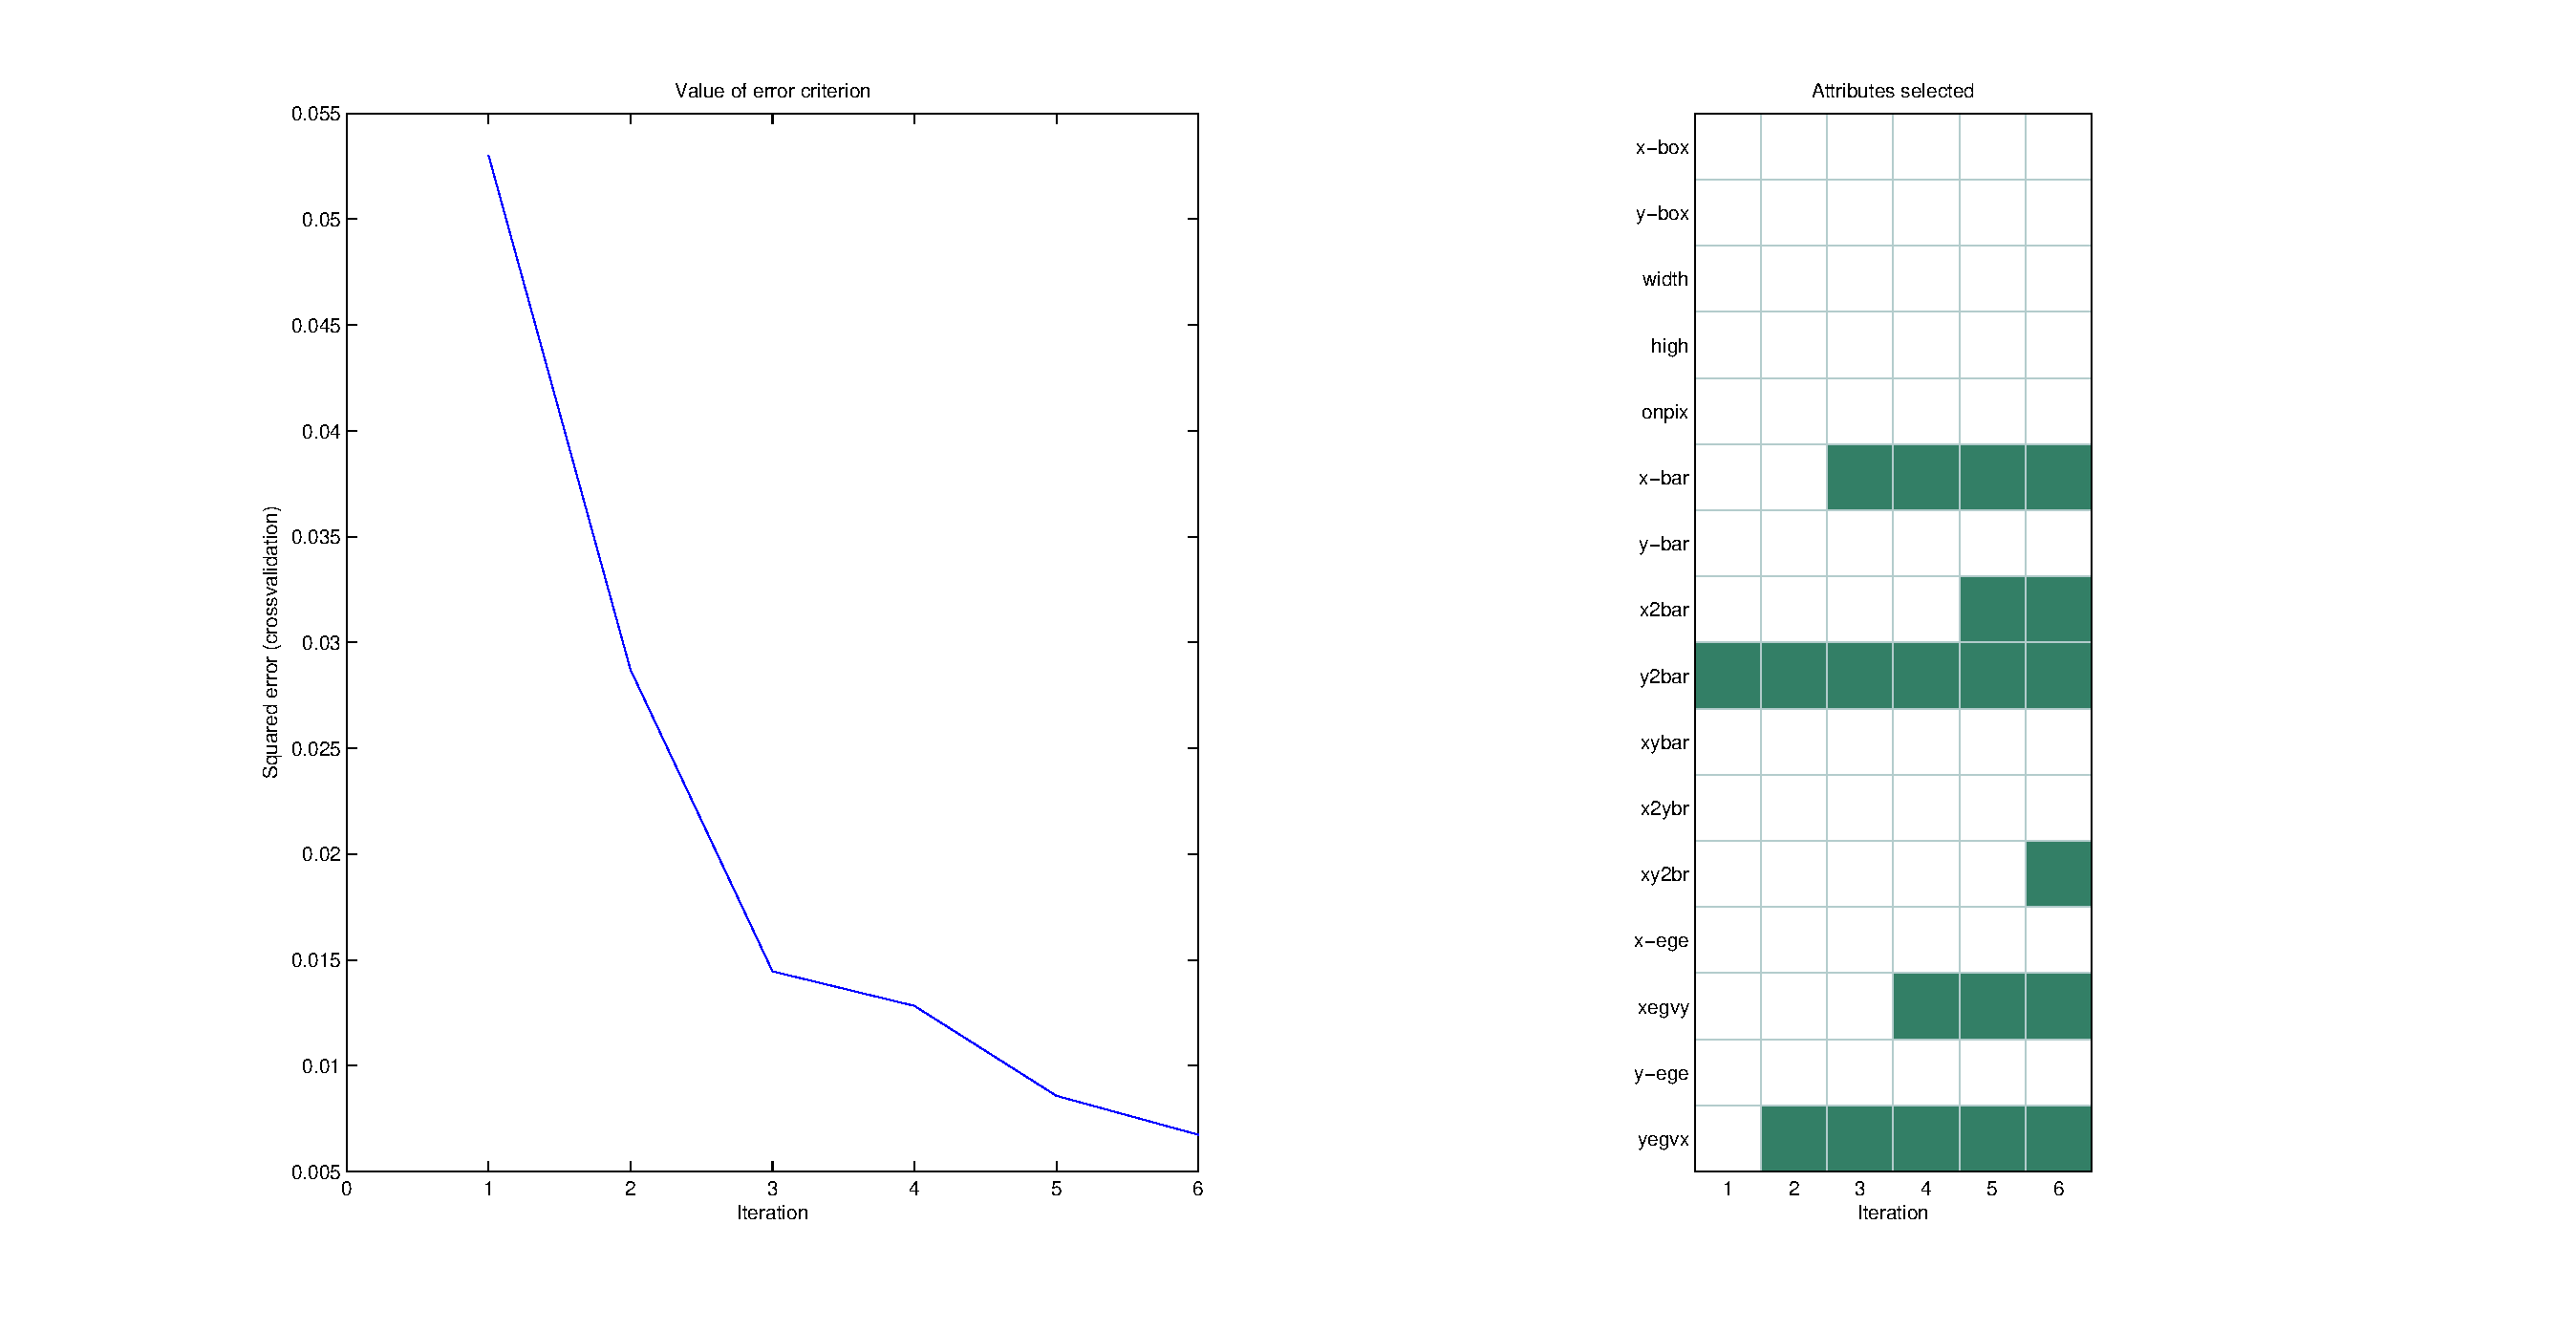
\includegraphics[width = 1.0\textwidth]{figure_p2/r2.eps}
\caption{Feature selection and crossvalidation error for fold 5}
\end{figure}

We also find that in almost all cases there is no significant performance improvement ($R^2$ test score) between selecting all the features and the features suggested by the feature selection:
\begin{verbatim}
Linear regression without feature selection:
- Training error:        0.00
- Test error:            0.01
- R^2 train:             0.99
- R^2 test:              0.95
Linear regression with sequential feature selection:
- Training error:        0.00
- Test error:            0.01
- R^2 train:             0.98
- R^2 test:              0.96
\end{verbatim}

However the feature selection allows to have a much simpler model with almost the same error performance.\\

Plotting the residual error vs. the attributes can give some insight into whether including a transformation of a variable can improve the model. If the points in a residual plot are randomly dispersed around the horizontal axis, a linear regression model is appropriate for the data; otherwise, a non-linear model is more appropriate.
Looking the residual plot in figure 1.3, it shows a random pattern which indicates a good fit for a linear model.
In fact, if we include transformation of some variable (for example the square of an attribute) we checked that there is no significant performance improvement.

\begin{figure}[htbp]
\center
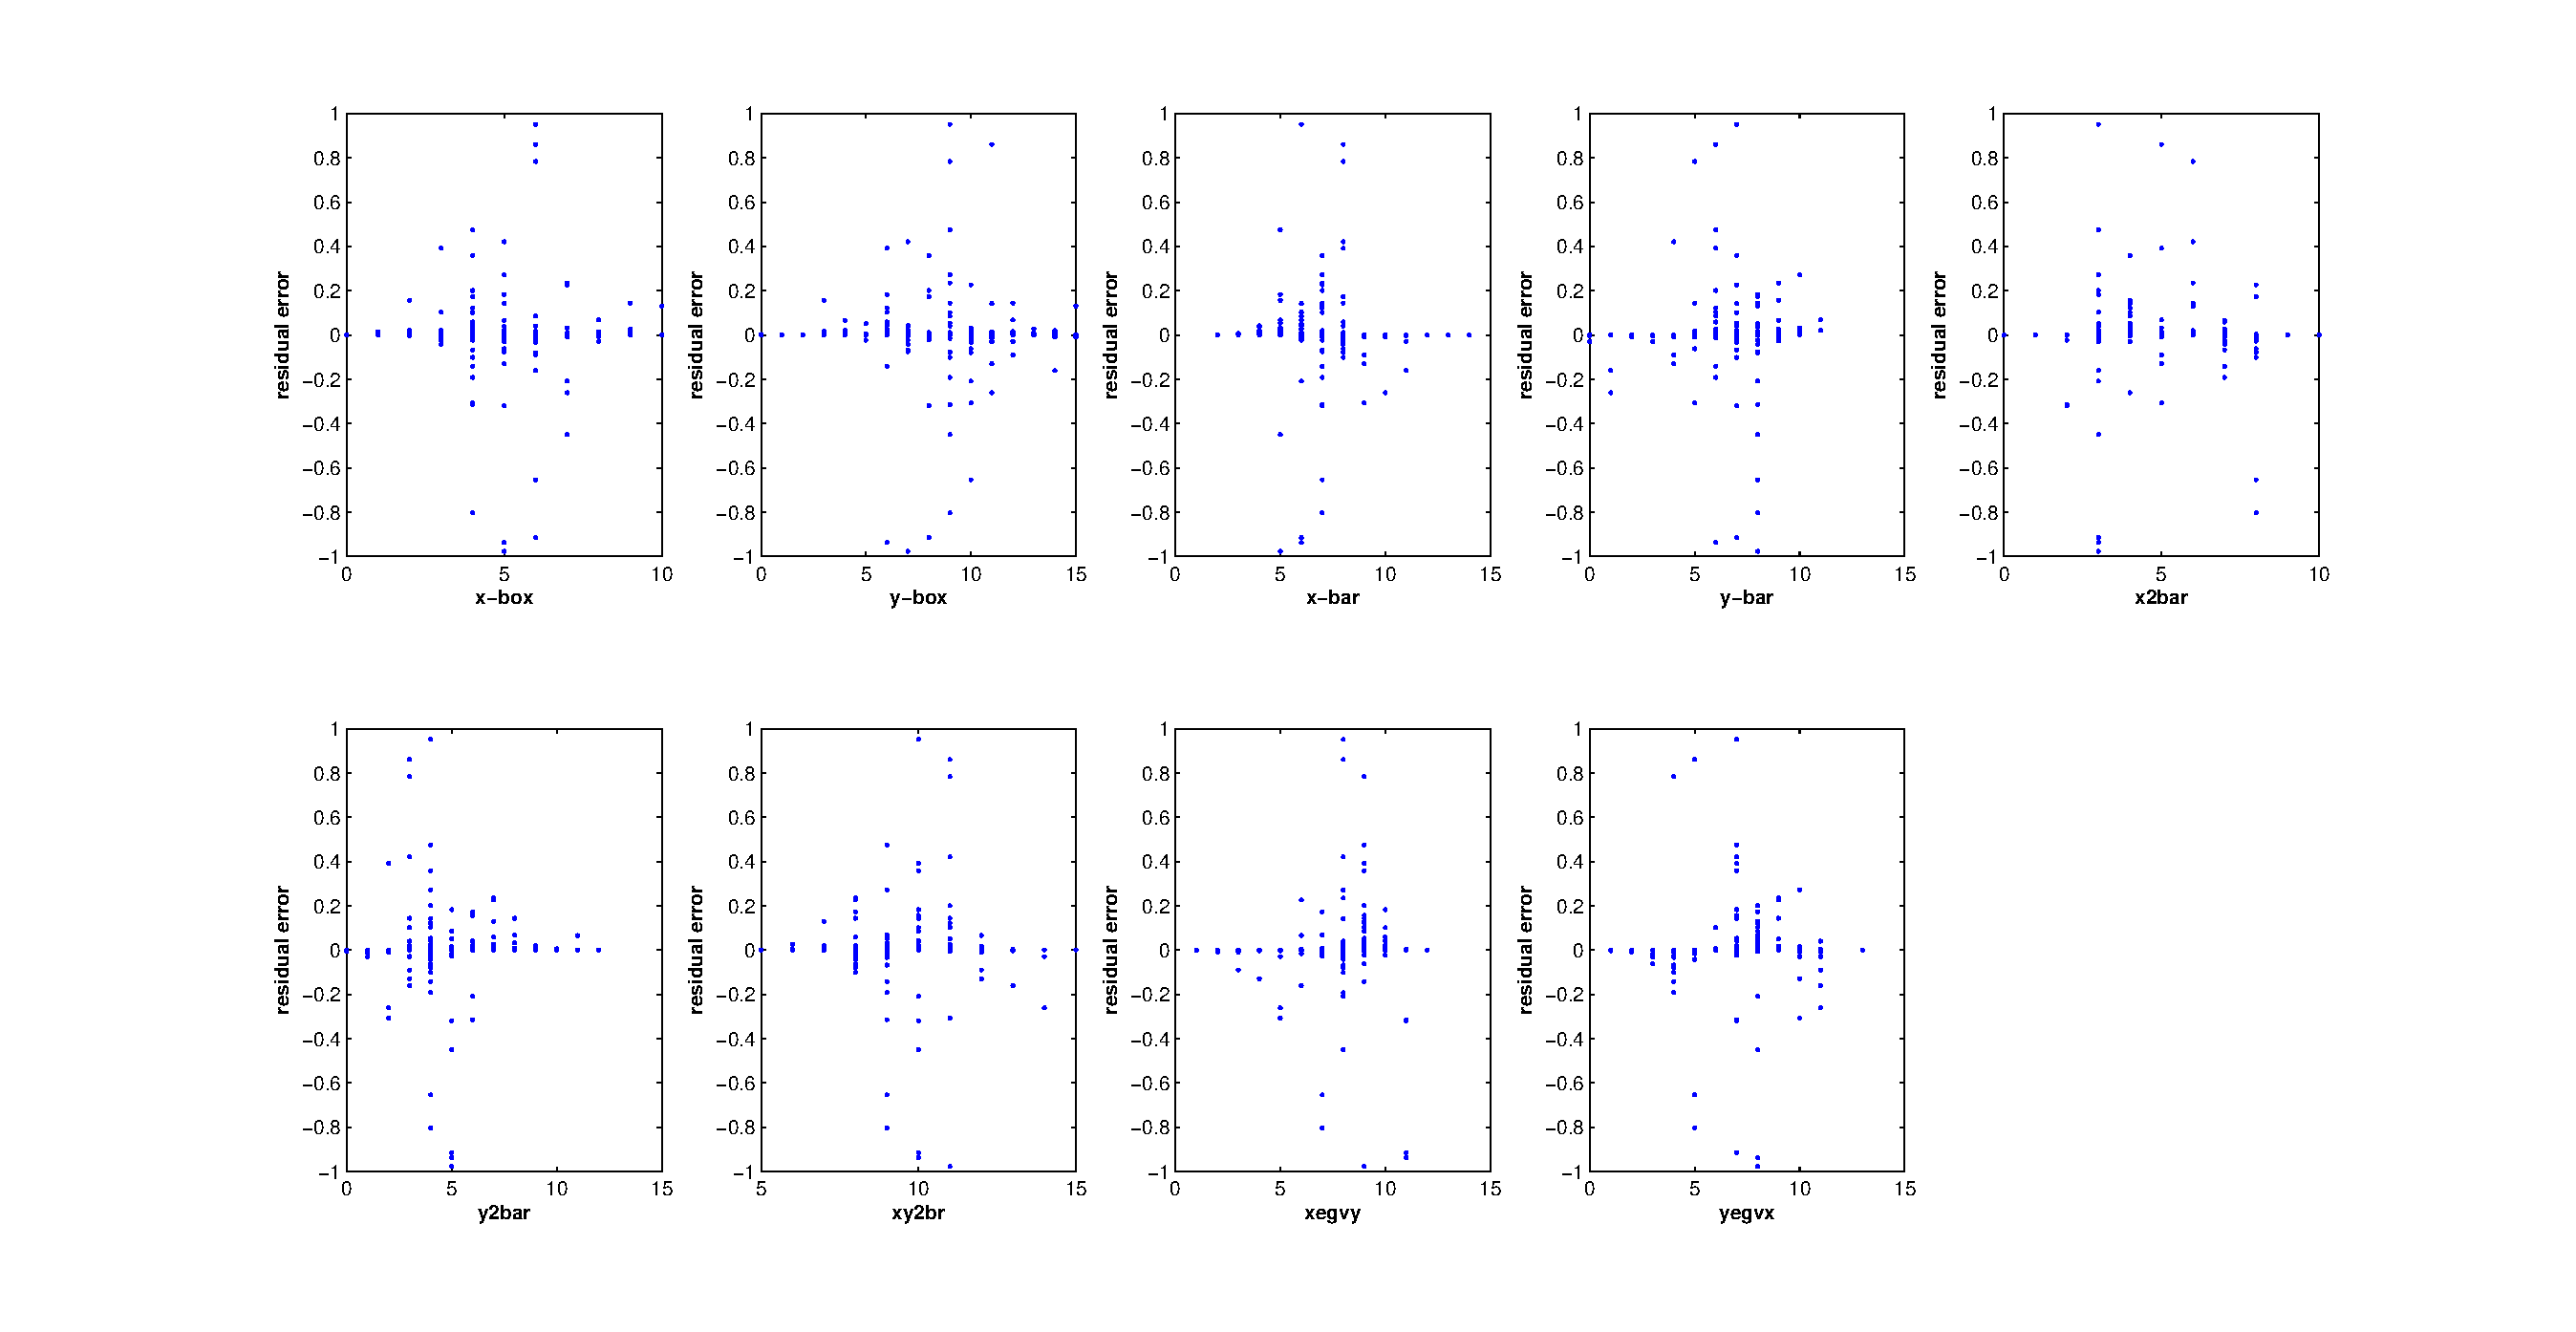
\includegraphics[width = 1.1\textwidth]{figure_p2/r3.eps}
\caption{Residual error vs. the attributes}
\end{figure}

\section*{Attributes effects}
Another approach to control for the complexity of the model is to regularize the parameters in the objective function. In linear regression we can regularize the parameter $\textbf{w}$ by the Frobenius norm. 
We run linear regression with regularization for the letter index attribute, with external 5-fold cross-validation and internal 10 fold cross-validation for estimating the optimal lambda value. Figure 1.4 shows that the optimal lambda = $10^{-2}$, and how the attribute weights change due to regularization.

\begin{figure}[htbp]
\center
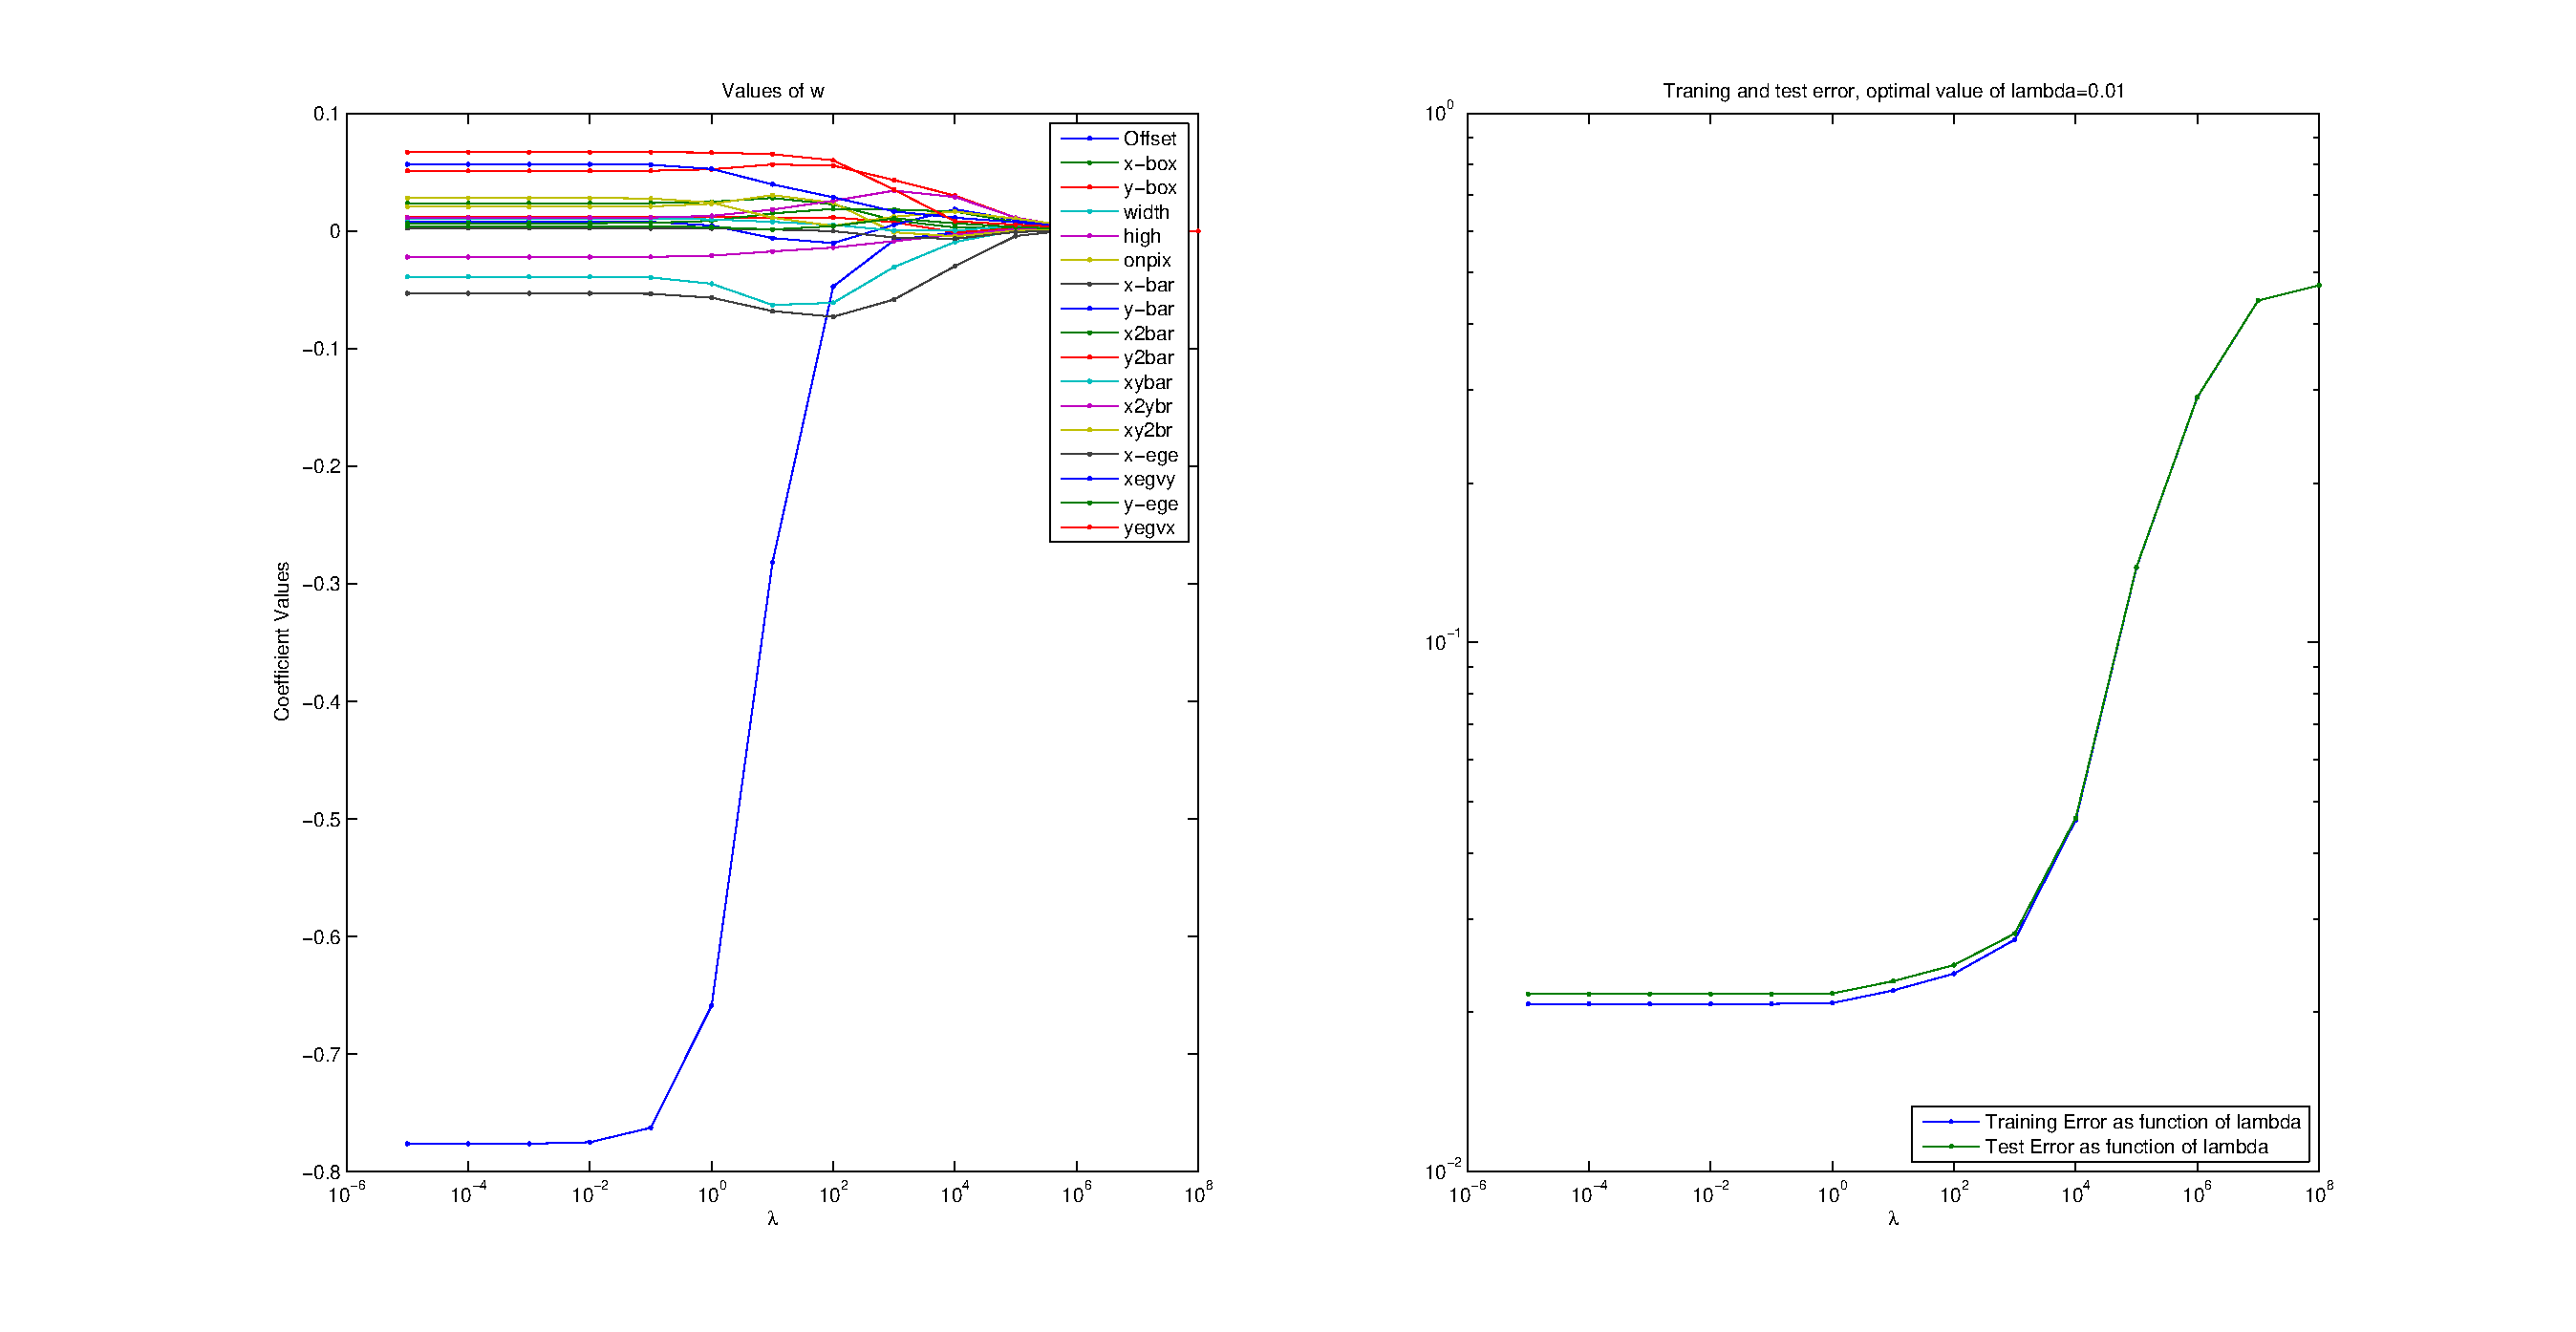
\includegraphics[width = 1.25\textwidth]{figure_p2/r5.eps}
\caption{Linear regression with regularization,  attribute weights and optimal $\lambda$}
\end{figure}

We calculate the average set of weights and we plot a bar chart to understand the contributions of the different attributes for the letter value [Figure 1.5]. We see again that in order x-bar, y2bar, xegvy, yegvx are the most significant predictors. 

\begin{figure}[htbp]
\center
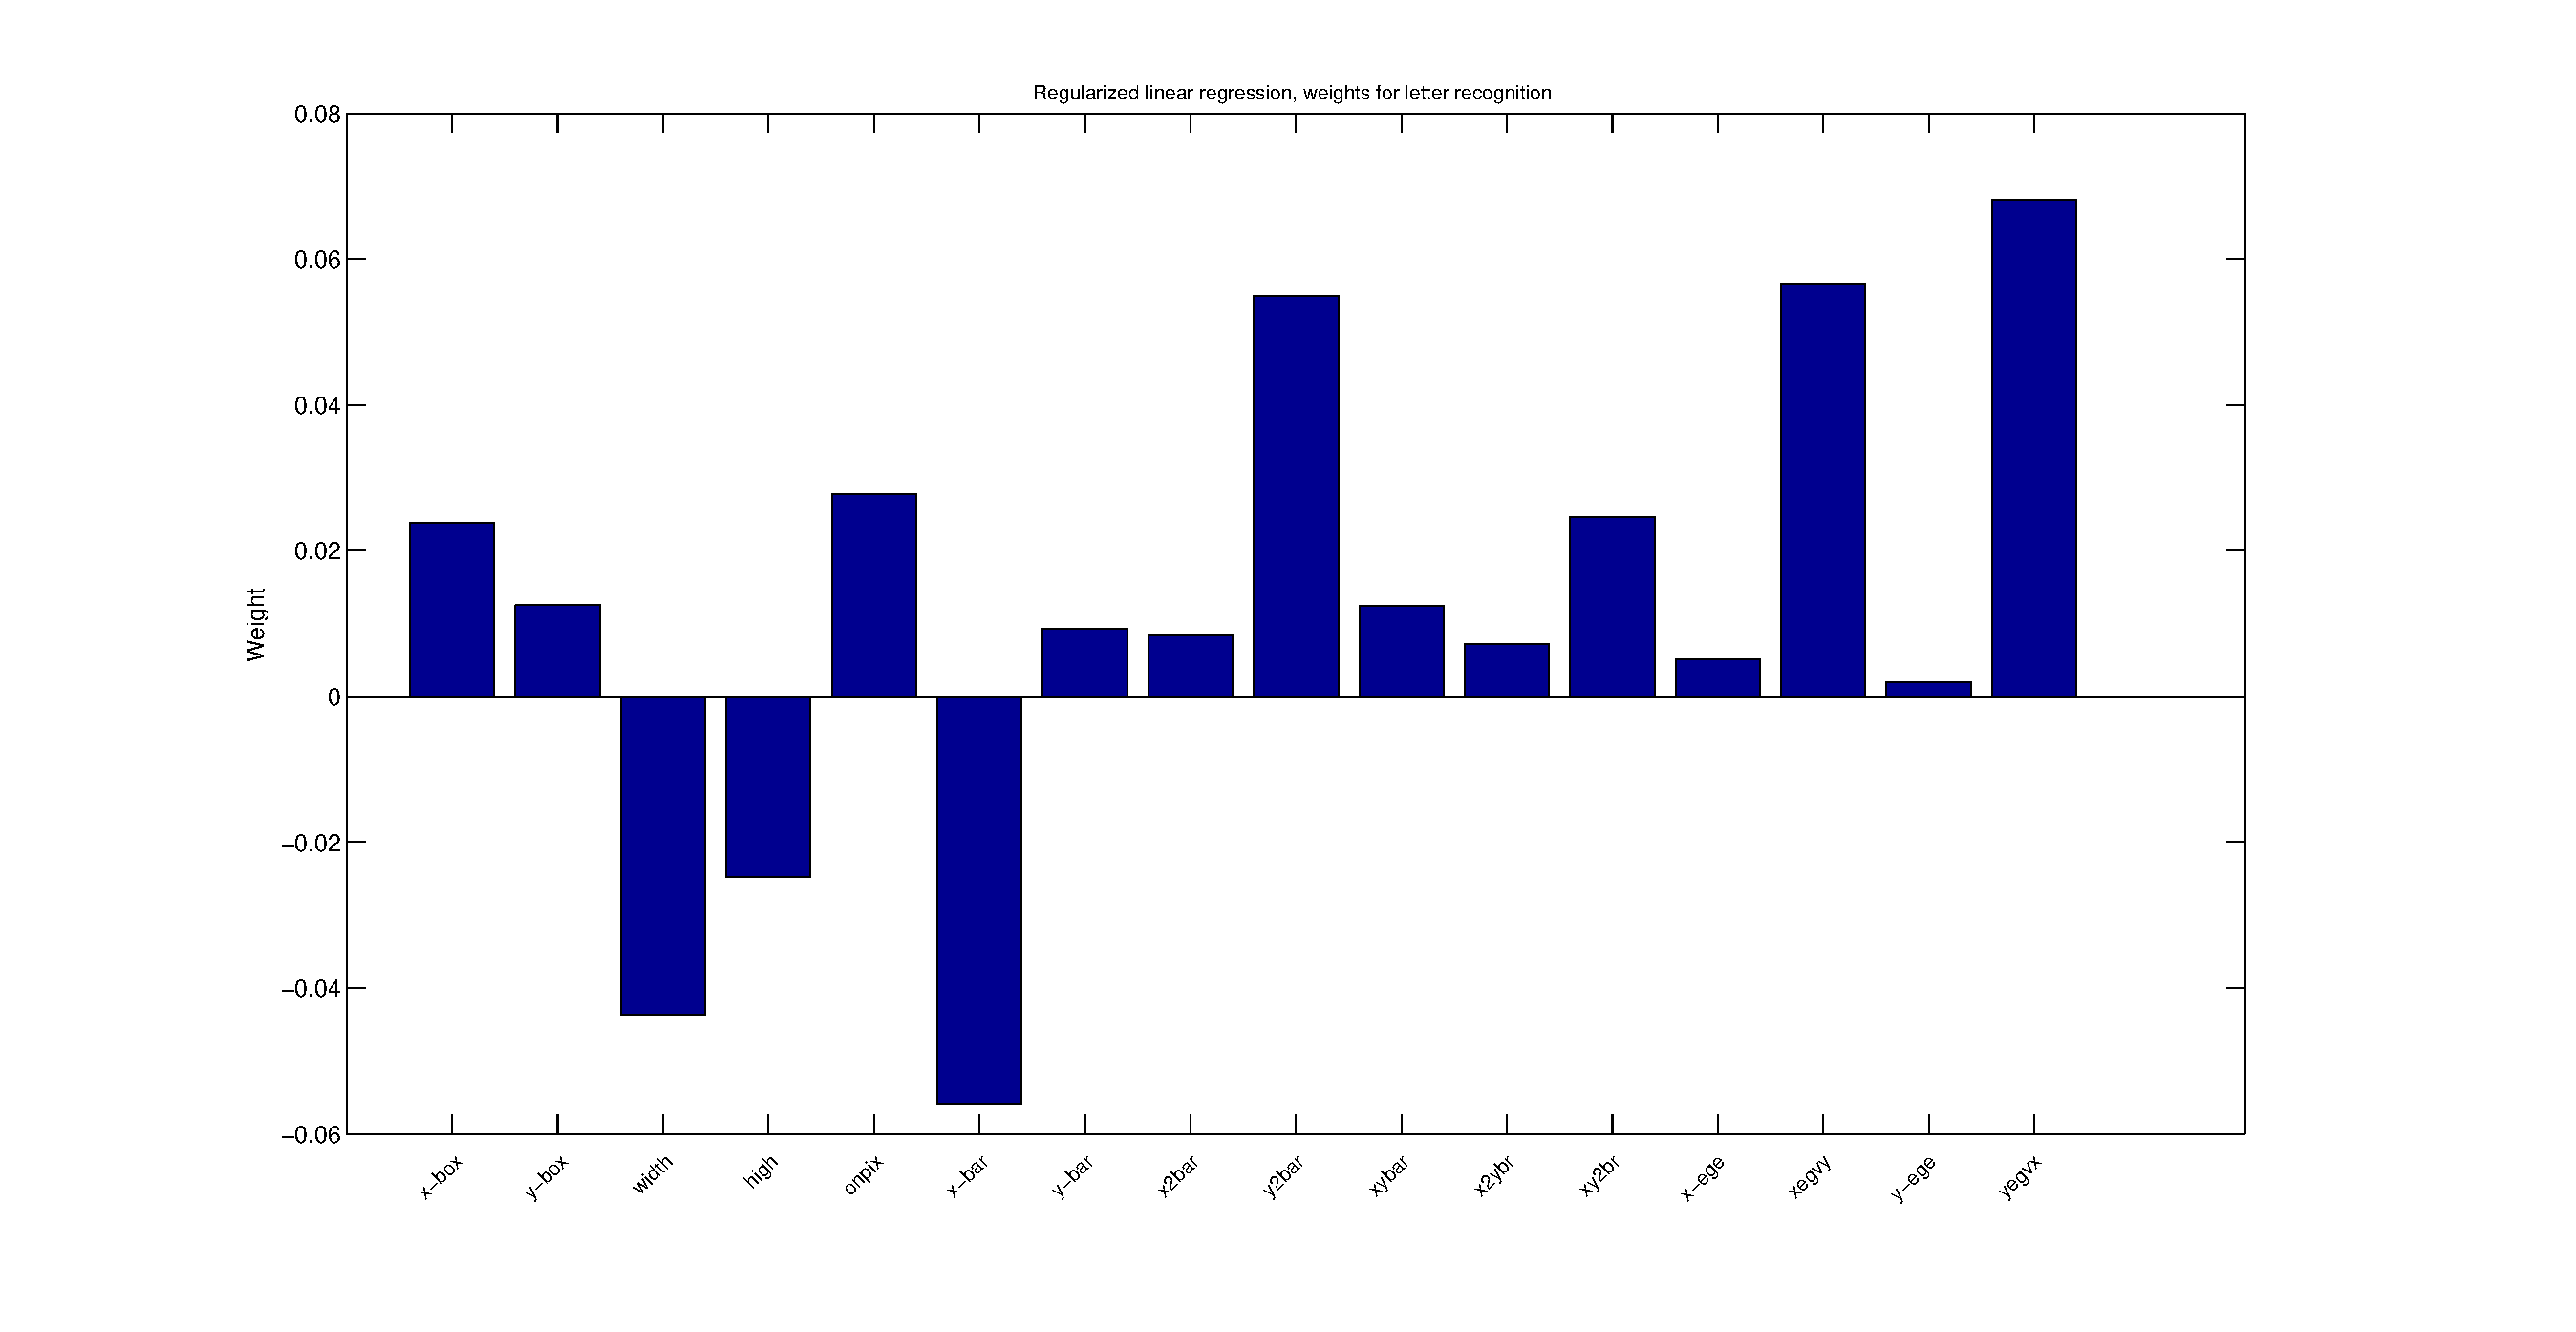
\includegraphics[width = 1.25\textwidth]{figure_p2/r6.eps}
\caption{Linear regression with regularization, attribute weights}
\end{figure}

The squared errors scores however show no significant improvement between the non regularized and the regularized models.

\section*{1.4 Artificial neural network}
We fit an artificial neural network (ANN) to the data. We perform a 5 fold cross-validation to select the number of hidden units hyper-parameter. For each fold, we try to fit an ANN 5 times, and we select the ANN which produces the lowest train error.
Just using only one hidden units and one train of neural network we obtain very interesting results, indeed, in this case, the train error and test error are approximately equal to 0\% and 1\% respectively. Increasing the number of re-train the errors remain pretty the same while increasing the number of hidden nodes (for instance equal to six), the train error and test error decrease and they are approximately equal to 0\% and 0\% (0.16\%) respectively.

Figure 1.5 describe an ANN with 16 inputs(attributes) and one hidden layer that we have chosen as model to fit our data.
\begin{figure}[htbp]
\center
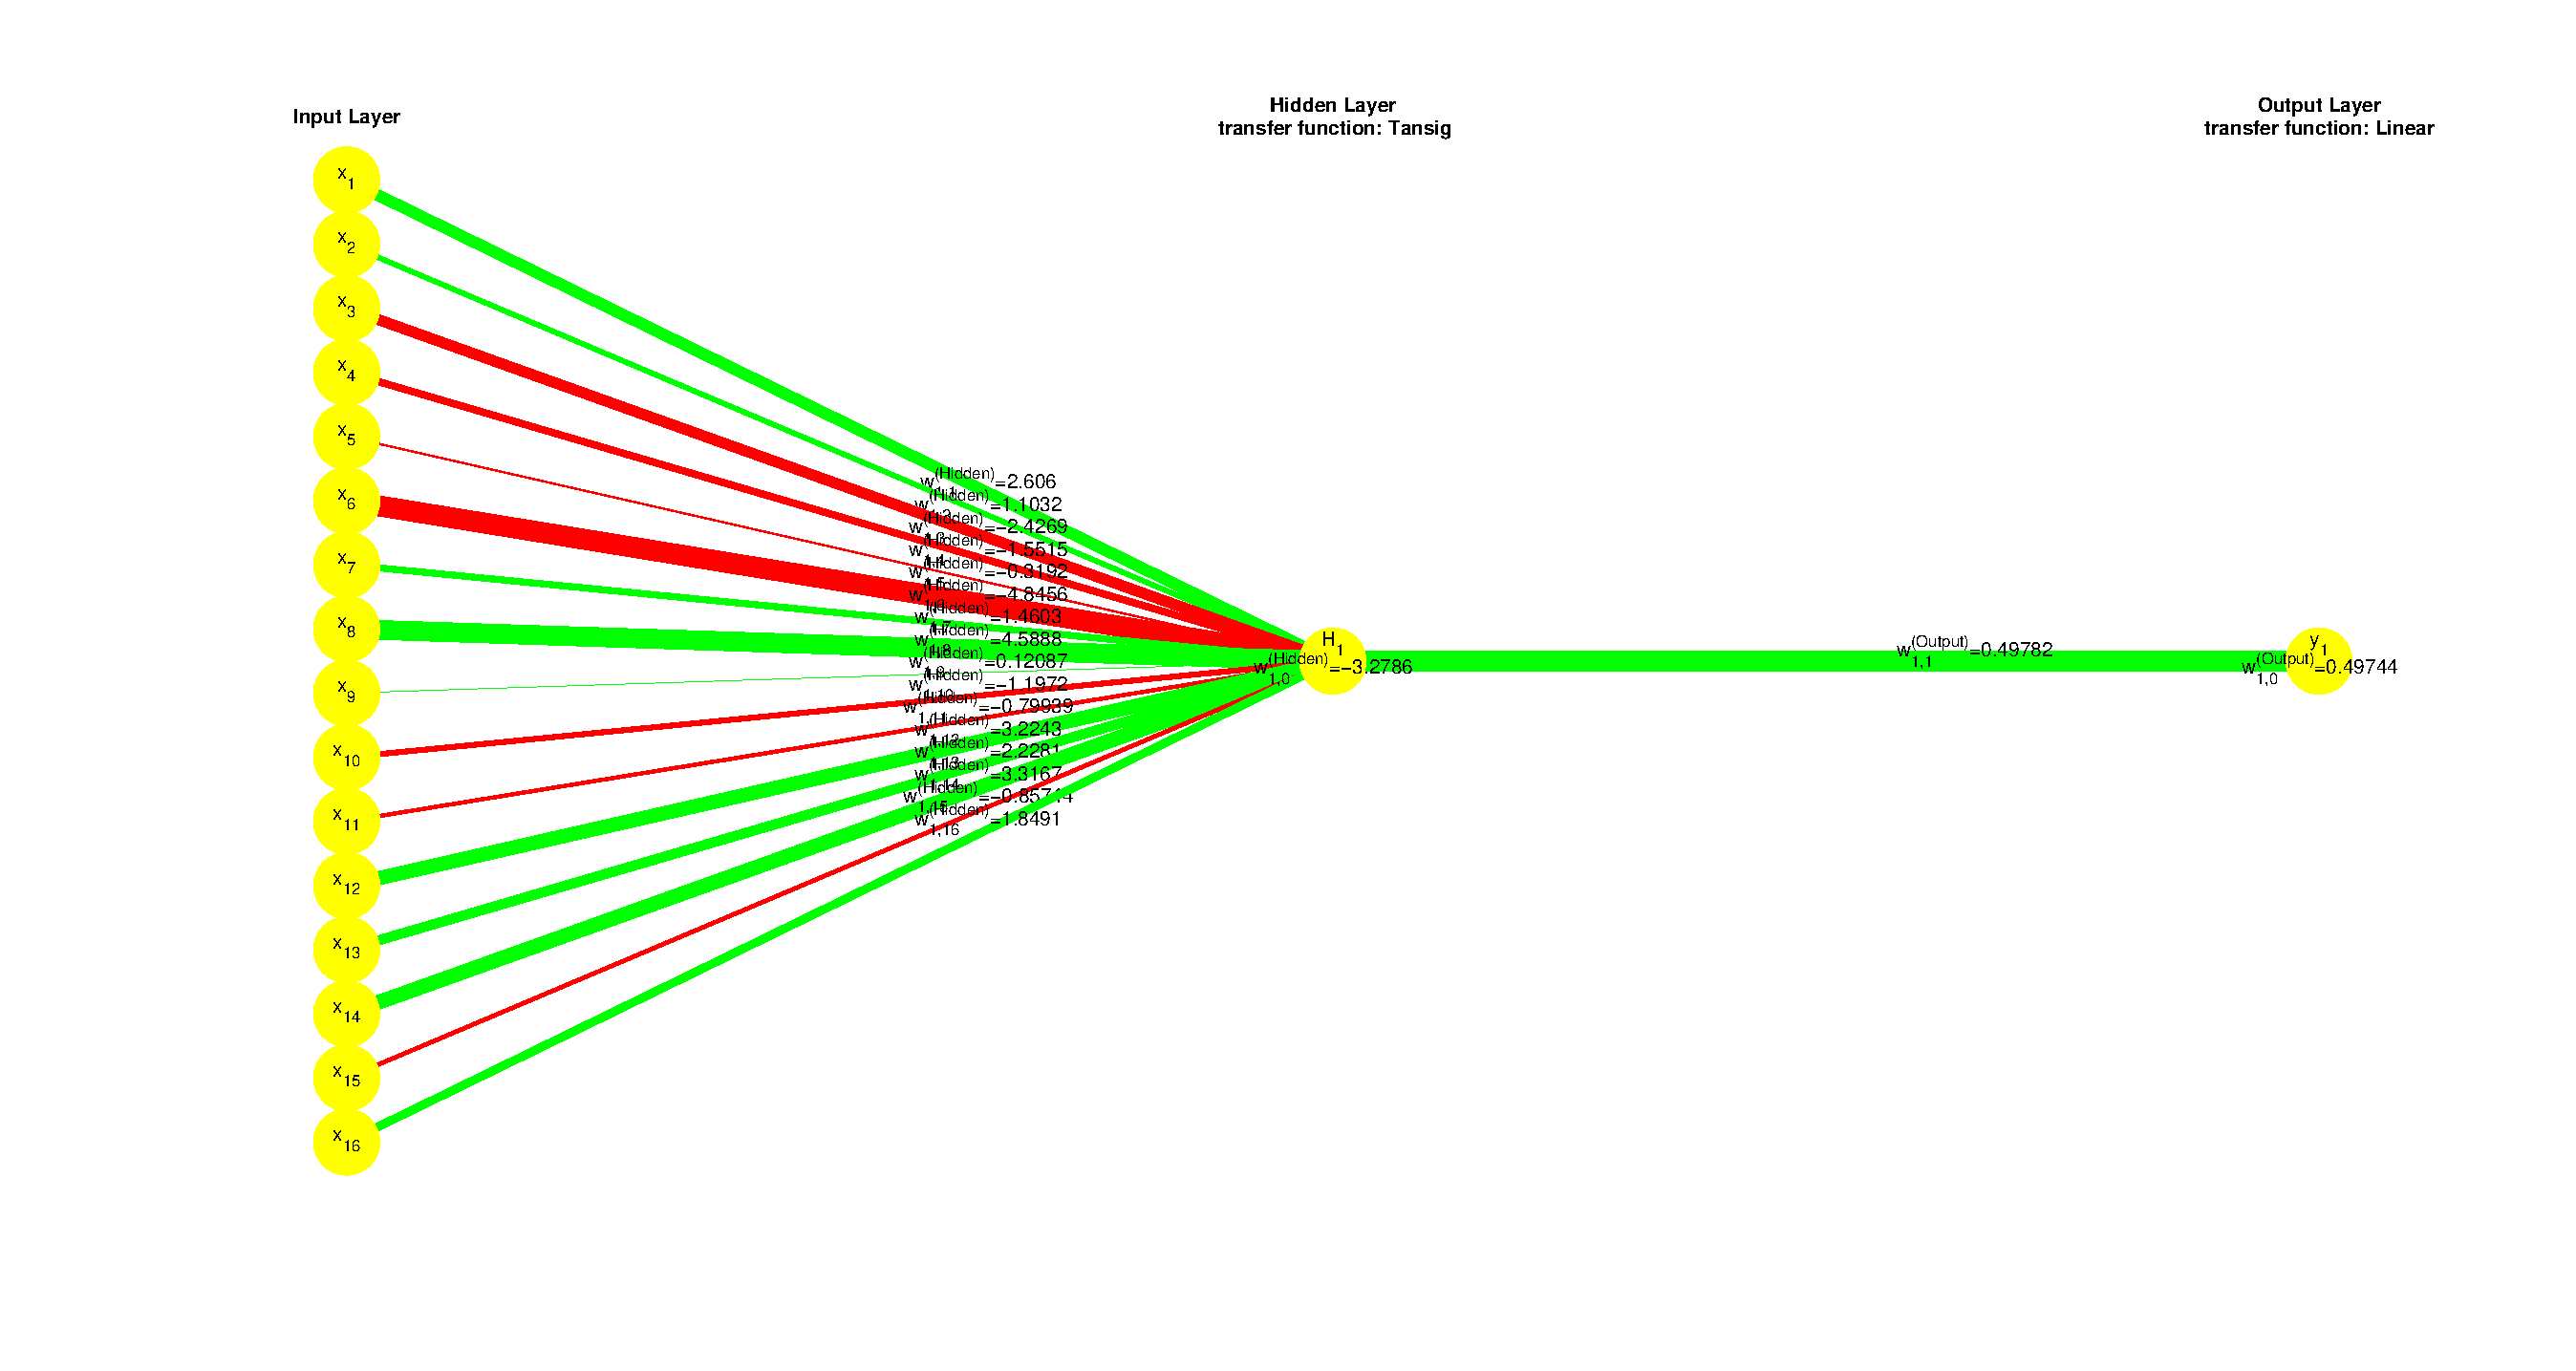
\includegraphics[width = 1.0\textwidth]{figure_p2/n1.eps}
\caption{ANN with one hidden unit}
\end{figure}


\section*{1.5 Comparison}
We perform a pairwise $t$-test between the regularized linear regression model, the ANN with one hidden node, and a baseline model predicting the average of the output variable (letter $A$ or $C$). In order to compare the models we consider the error rate average of the five folds. 
\begin{verbatim}
- Error rate linear regression      0.9%
- Error rate ANN                    1.1%
- Error rate predict average        48.3%
\end{verbatim}
If we compare Linear regression vs ANN we note that the classifiers are NOT significantly different while if we compare linear regression vs predict average and ANN vs predict average it easy understand that the classifiers are significantly different. We can see the results also in Figure 1.7.

\begin{figure}[htbp]
        \center
       	\begin{subfigure}[a]{0.35\textwidth}
                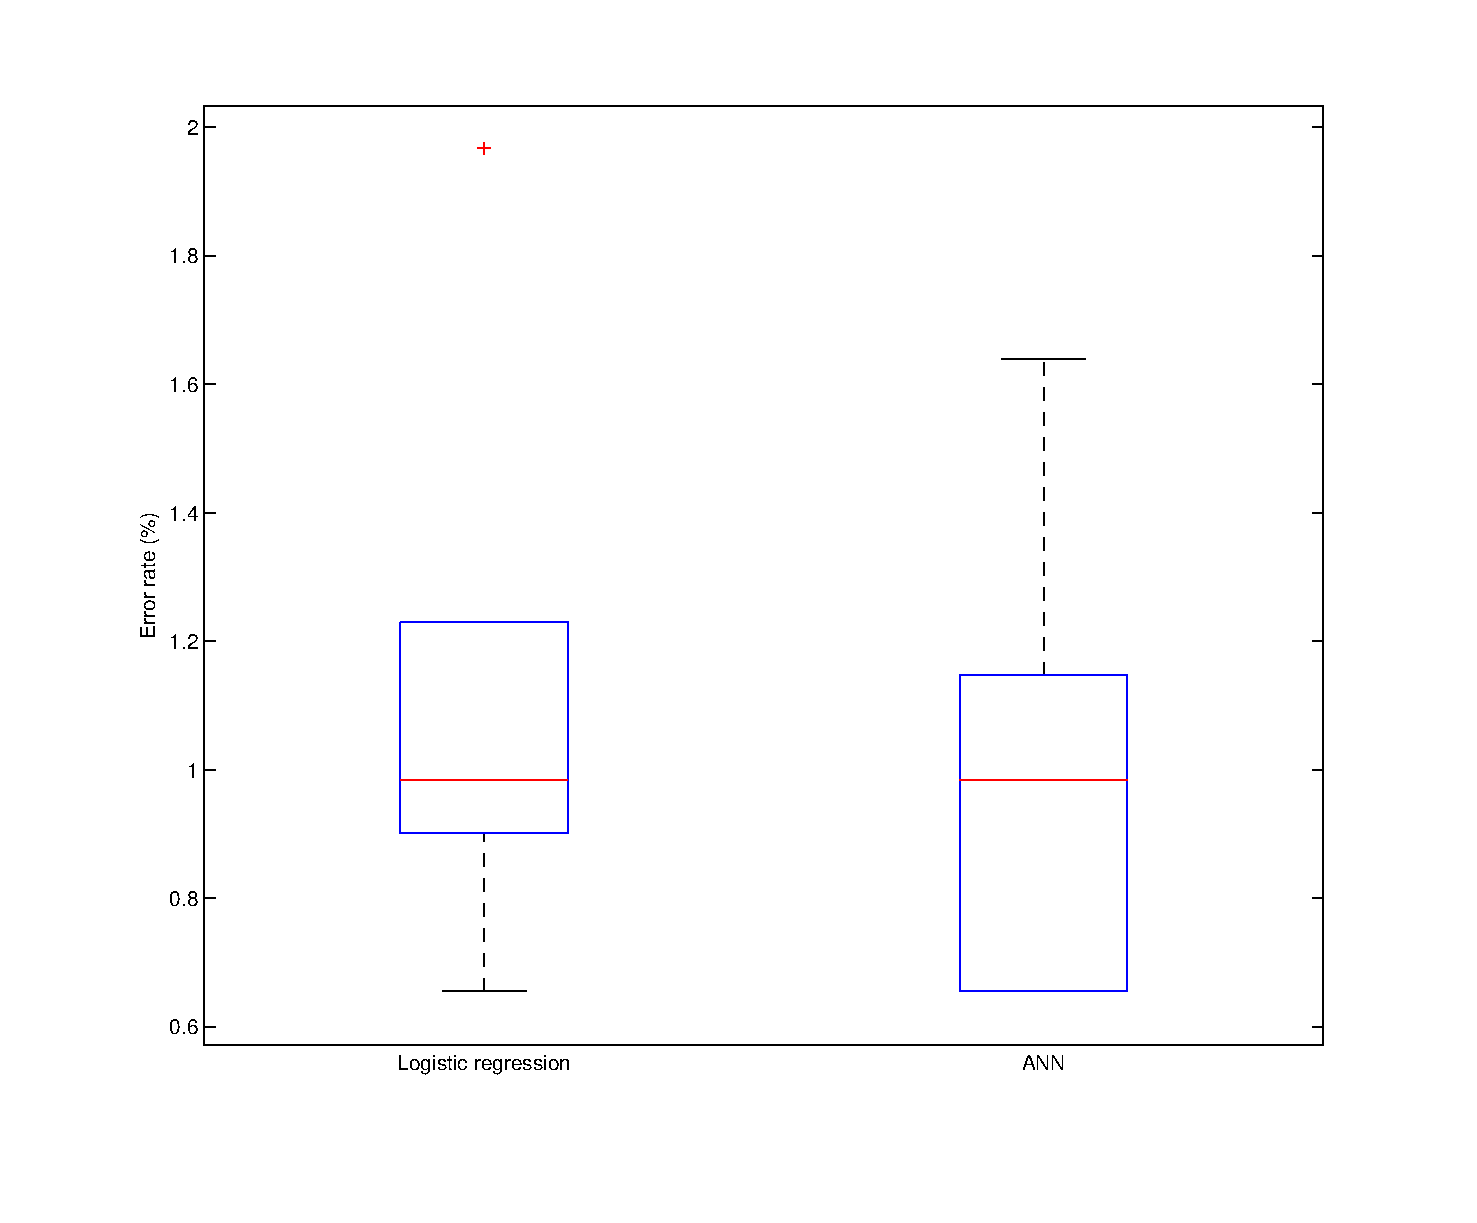
\includegraphics[width=4.8cm]{figure_p2/c1.eps}
                \caption{Linear Regression vs ANN}
        \end{subfigure}%
        \begin{subfigure}[b]{0.35\textwidth}
                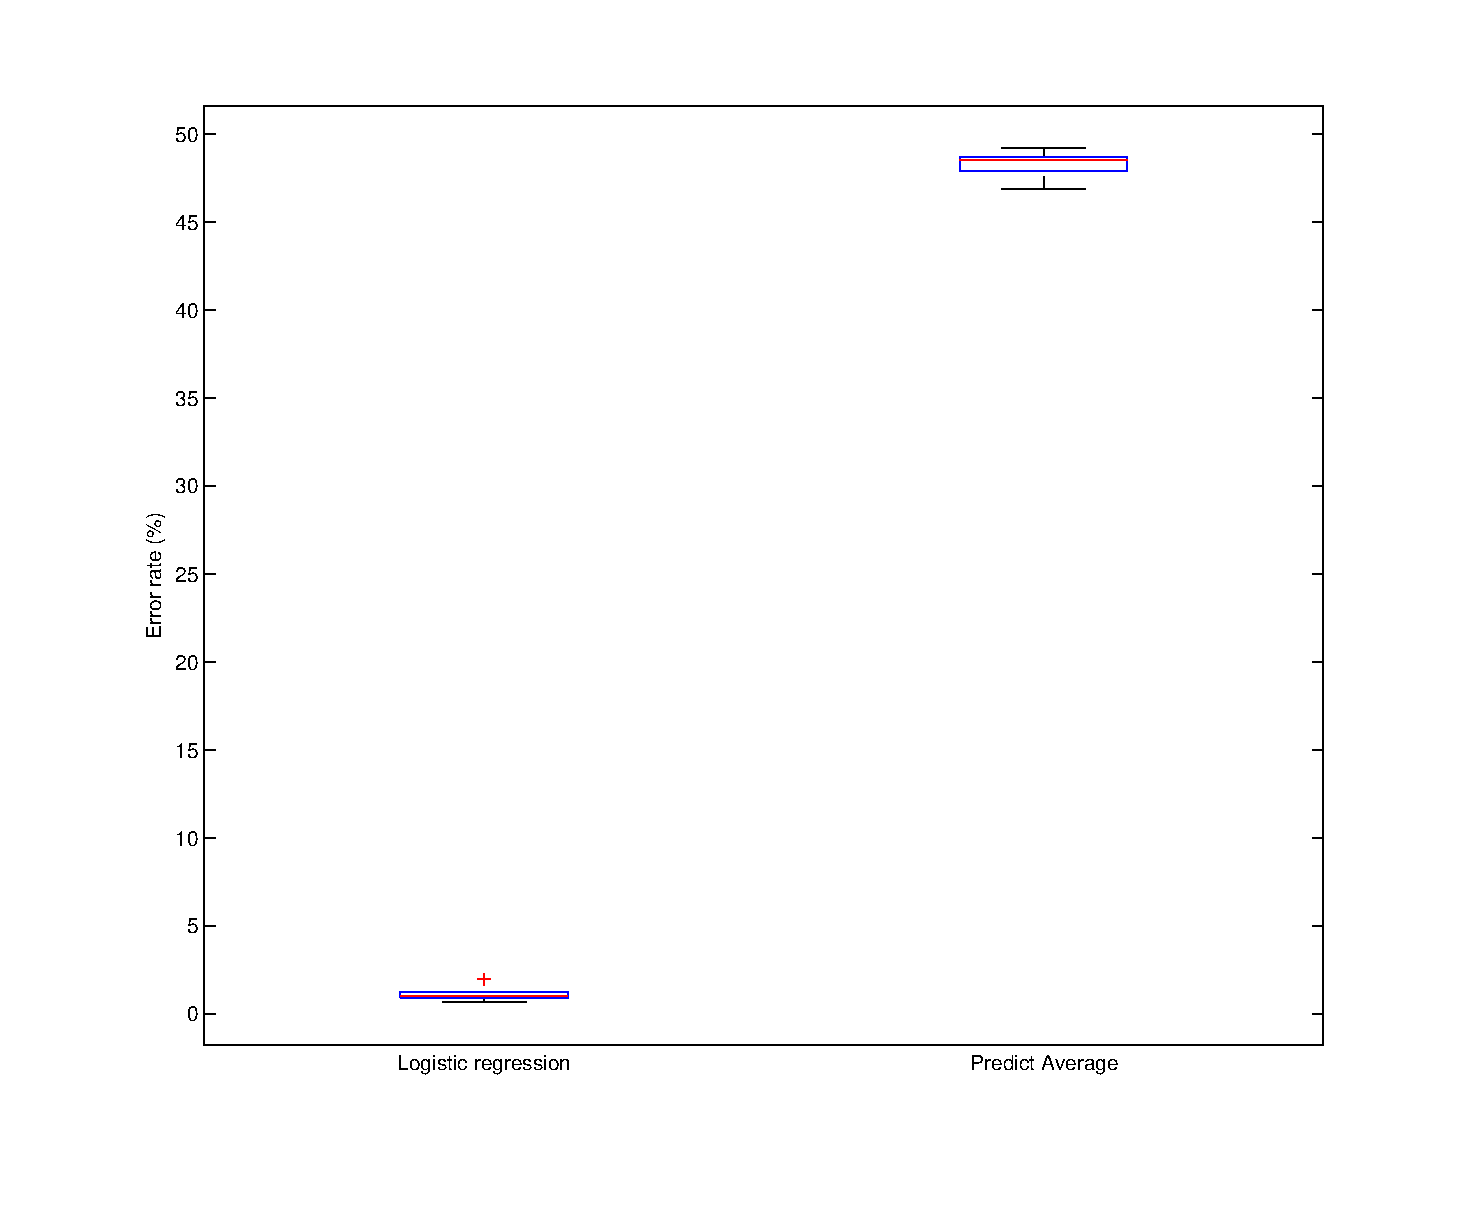
\includegraphics[width=4.8cm]{figure_p2/c2.eps}
                \caption{Linear Regression vs Predict Average}
                 \end{subfigure} \\

         \begin{subfigure}[c]{0.35\textwidth}
                \centering
                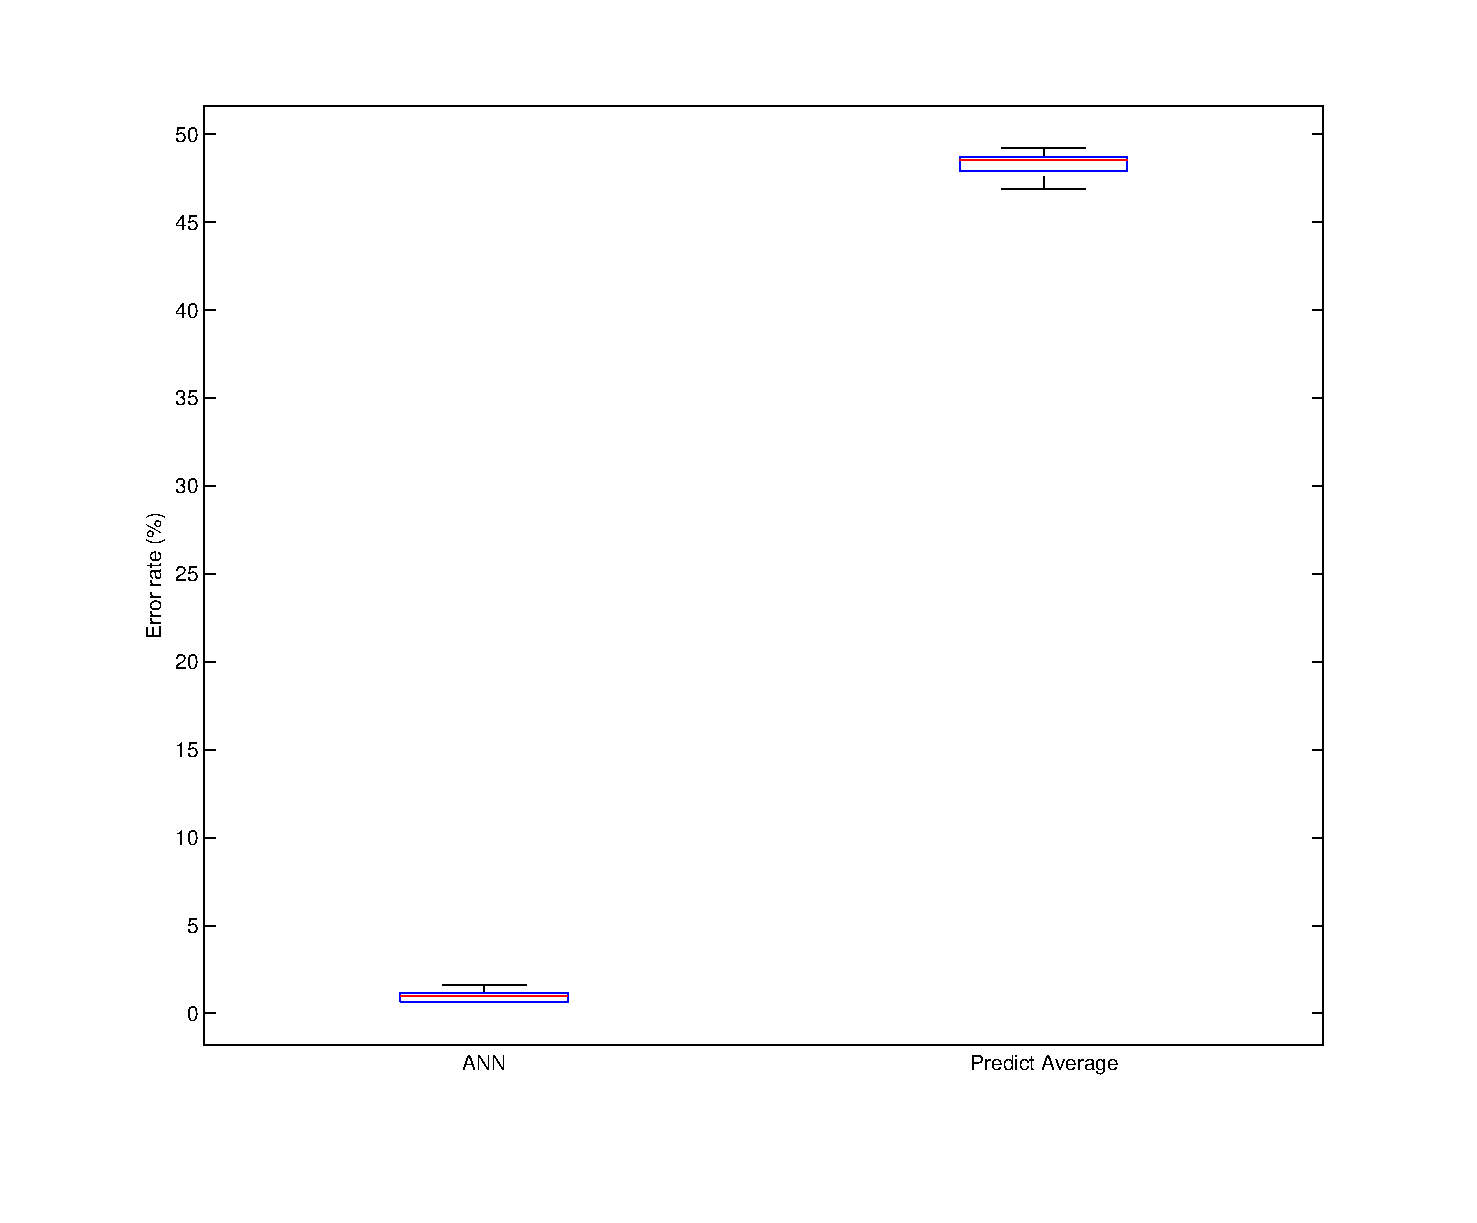
\includegraphics[width=4.8cm]{figure_p2/c3.eps}
                \caption{ANN vs Predict Average}
        \end{subfigure}
        \caption{Box-Plots: Permormace of the models one against the other}
\end{figure}

\section*{MULTI-CLASS LOGISTIC REGRESSION}
We run multi-class classification data set which fits logistic regression models to the training data using the one-against-rest strategy (each classifier trained to predict one class label vs. the remaining). Next, it computes the outputs of the C classifiers on the test data and classifies it according to the highest output.
Our goal is classify, using multi-class regression model, all the letter indexes. 

We use $\frac{2}{3}$ of the data set as training set and the remainder data for the test set and we obtain an error rate equals to 28\%.
Always considering the one-against-rest scheme, we fit 26 (number of outputs) neural networks with 2 hidden units. We use $\frac{2}{3}$ of the data set as training set and the remainder data for the test set and we obtain an error rate equals to 25\%.
Instead, considering a predict average model for all the 26 letters we obtain an error rate equals to 98\%. 
Comparing these results we can say, even in multi-class classification, that the performance of multi-class regression vs multi-class ANN are not significantly different while if we consider predict average model vs regression or ANN obviously the performance are significantly different. This happens because predict average model is very inefficient when the number of classes is high.
